%! Author = antonio
%! Date = 7/2/24

\subsubsection{Linear Support Vector Machines}
Support Vector Machines are linear classifiers that look for maximum margin separation hyperplanes.
The primal formulation of the soft-margin SVM problem consists in minimizing the function:

\begin{equation}
    \mathbf{J}(w,b)= \frac{1}{2}||w||^2 + C\sum_{i=1}^{N}max(0,1-z_i(w^Tx_i+b))
    \label{eq:SVMprimalFormulation}
\end{equation}

where in \autoref{eq:SVMprimalFormulation} N is the number of training samples, C is the regularization parameter,
and \(z_i\) is the margin of the i-th sample.\\
The dual formulation of the problem is:

\begin{equation}
    \mathbf{J}(\alpha)= - \frac{1}{2} \alpha^T \;\textbf{H} \;\alpha + \alpha^T \textbf{1} \;\;\;\;\;\;1\leq \alpha_i\leq C,\;\; \forall i \in \{1,...,N\},\;\; \sum_{i=1}^{n}\alpha_i z_i=0
    \label{eq:SVMdualFormulation}
\end{equation}

where H in  \autoref{eq:SVMdualFormulation} is \(H_{ij}=z_iz_jx_i^Tx_j\) and the dual solution is the maximizer of \(J^D(\alpha)\).\\
Primal and dual solutions are related through:

\begin{equation}
    w^*=\sum_{i=1}^{N}\alpha_i^* z_i x_i
\end{equation}

In addition it's possible to rewrite dual problem as minimization of:
\begin{equation}
    \hat{\mathbf{L}}(\alpha)=-\mathbf{J}(\alpha)= \frac{1}{2} \alpha^T \;\textbf{H} \;\alpha - \alpha^T \textbf{1}
\end{equation}

and it can be minimized by L-BFGS-B algorithm.
After that we have calculated the optimal \(\alpha\) we can compute \(w^*\).

\begin{figure}[h!]
    \centering
    \begin{subfigure}[b]{0.30\linewidth}
        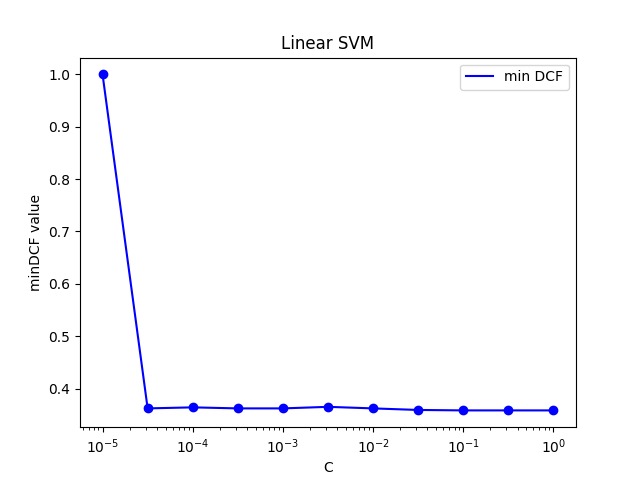
\includegraphics[width=\linewidth]{Lab/09. Lab 09/Images/01. L - minDCF}
        \label{fig:LminDCF}
    \end{subfigure}
    \begin{subfigure}[b]{0.30\linewidth}
        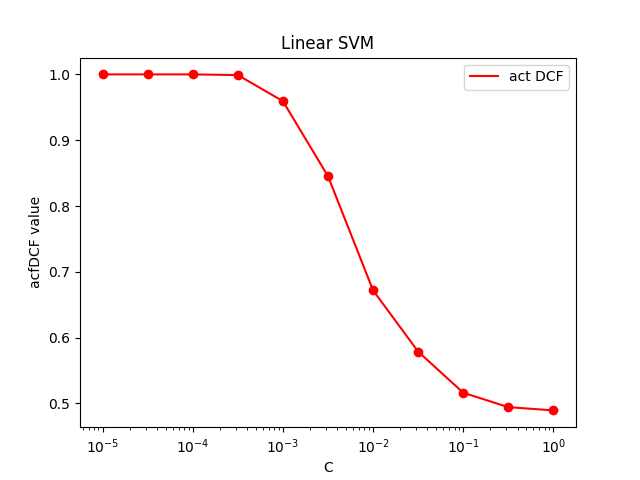
\includegraphics[width=\linewidth]{Lab/09. Lab 09/Images/02. L - actDCF}
        \label{fig:LactDCF}
    \end{subfigure}
    \begin{subfigure}[b]{0.30\linewidth}
        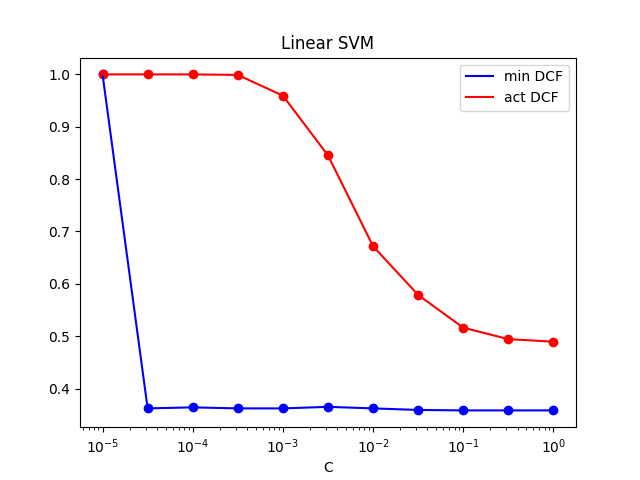
\includegraphics[width=\linewidth]{Lab/09. Lab 09/Images/03. L - min And actDCF}
        \label{fig:LminAndActDCF}
    \end{subfigure}
    \caption{Shows minDCF and actDCF for Linear SVM}
    \label{fig:LSVM}
\end{figure}

\begin{table}[h!]
    \centering
    \begin{tabular}{>{\centering\arraybackslash}p{2.5cm} >{\centering\arraybackslash}p{2.5cm} >{\centering\arraybackslash}p{2.5cm}}
        \toprule
        \multicolumn{3}{c}{\textbf{Linear SVM \(K=1.0\)}} \\
        \midrule
        \texbf{C}   & \textbf{minDCF} & \textbf{actDCF} \\
        \midrule
        \(10^{-5}\) & 1.0000          & 1.0000          \\
        \(10^{-4}\) & 0.3640          & 1.0000          \\
        \(10^{-3}\) & 0.3620          & 0.9593          \\
        \(10^{-2}\) & 0.3620          & 0.6718          \\
        \(10^{-1}\) & 0.3582          & 0.5162          \\
        \(10^{0}\)  & 0.3582          & 0.4894          \\
        \bottomrule
    \end{tabular}
    \captionsetup{justification=justified,singlelinecheck=false,format=hang}
    \caption{Show minDCF and actDCF for Linear SVM}
    \label{tab:SVMLin}
\end{table}

\newpage

\subsubsection{Kernel Support Vector Machines}
It's possible in Support Vector Machines to use kernels to allow nonlinear classification.
In this case there is no explicit expansion of the feature space;
we only can calculate the scalar product between the expanded features:\( k(x_1,x_2)=\phi(x_1)_T\phi(x_2)\) where k is the kernel function.
To do this we need to go and replace H as we saw in the previous section with \(\hat{H}= z_iz_jk(x_1,x_2)\).
During our project we see two different types of kernels:
\begin{itemize}
    \item \textbf{Polynomial kernel of degree d}: \(k(x_1,x_2)=(x_1^Tx_2+c)^d\)
    \item \textbf{Radial Basis Function kernel(RBF)}: \(k(x_1,x_2)=e^{-\gamma||x1-x_2||^2}\)
\end{itemize}
We can now apply the polynomial kernel to the SVM with \(d=2,\;\; c=1, \;\;\xi=0\) and see how minDCF and actDCF vary as C changes
in \autoref{fig:PolySVM} and \autoref{tab:SVMPoly}.

\begin{figure}[h!]
    \centering
    \begin{subfigure}[b]{0.30\linewidth}
        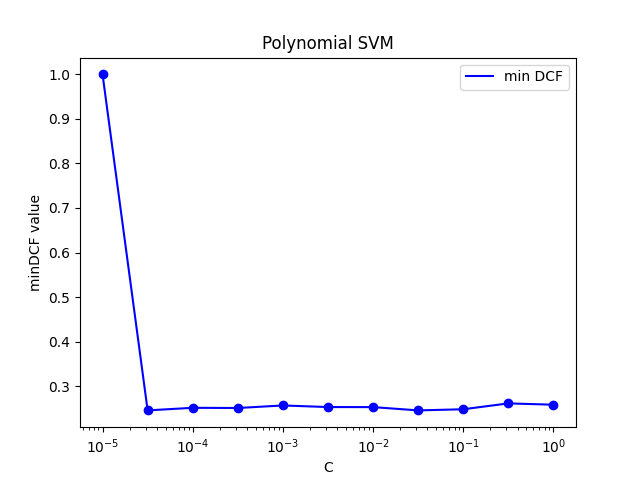
\includegraphics[width=\linewidth]{Lab/09. Lab 09/Images/04. Poly - minDCF}
        \label{fig:PolyminDCF}
    \end{subfigure}
    \begin{subfigure}[b]{0.30\linewidth}
        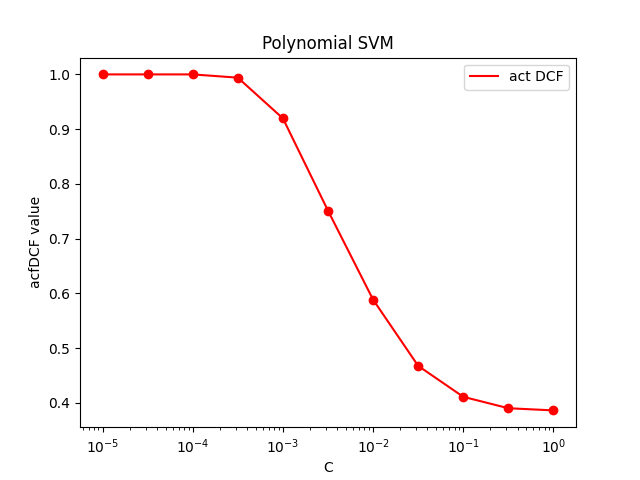
\includegraphics[width=\linewidth]{Lab/09. Lab 09/Images/05. Poly - actDCF}
        \label{fig:PolyactDCF}
    \end{subfigure}
    \begin{subfigure}[b]{0.30\linewidth}
        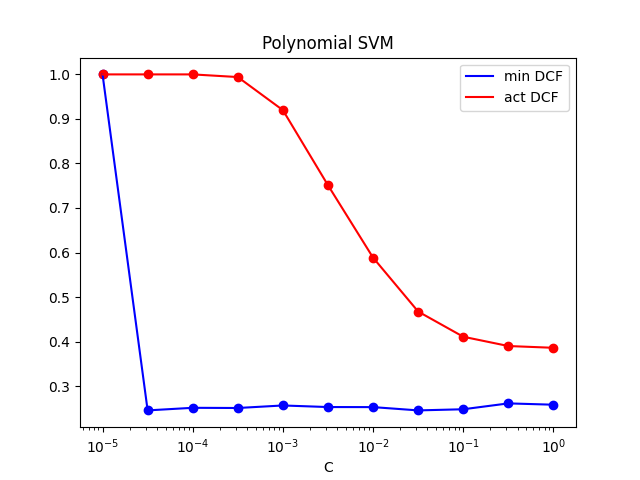
\includegraphics[width=\linewidth]{Lab/09. Lab 09/Images/06. Poly - min And actDCF}
        \label{fig:PolyminAndActDCF}
    \end{subfigure}
    \caption{Shows minDCF and actDCF with polynomial kernel}
    \label{fig:PolySVM}
\end{figure}


\begin{table}[h!]
    \centering
    \begin{tabular}{>{\centering\arraybackslash}p{2.5cm} >{\centering\arraybackslash}p{2.5cm} >{\centering\arraybackslash}p{2.5cm}}
        \toprule
        \multicolumn{3}{c}{\textbf{Polynomial Kernel \(d=2, c=1, \xi = 0\)}} \\
        \midrule
        \texbf{C}   & \textbf{minDCF} & \textbf{actDCF} \\
        \midrule
        \(10^{-4}\) & 0.2513          & 1.0000          \\
        \(10^{-3}\) & 0.2565          & 0.9196          \\
        \(10^{-2}\) & 0.2528          & 0.5884          \\
        \(10^{-1}\) & 0.2480          & 0.4109          \\
        \(10^{0}\)  & 0.2582          & 0.3861          \\
        \bottomrule
    \end{tabular}
    \captionsetup{justification=justified,singlelinecheck=false,format=hang}
    \caption{Show minDCF and actDCF for SVM with polynomial kernel}
    \label{tab:SVMPoly}
\end{table}

In this case apply a RBF kernel to the SVM with \(\xi=1\), the first thing we consider is which value of \(\gamma\) can
give us a better outcome in terms of minDCF and actDCF.
Looking at \autoref{fig:RadialSVM}, we sse that the best solution is given to us by \(\gamma=0.1\).

\begin{figure}[h!]
    \centering
    \begin{subfigure}[b]{0.40\linewidth}
        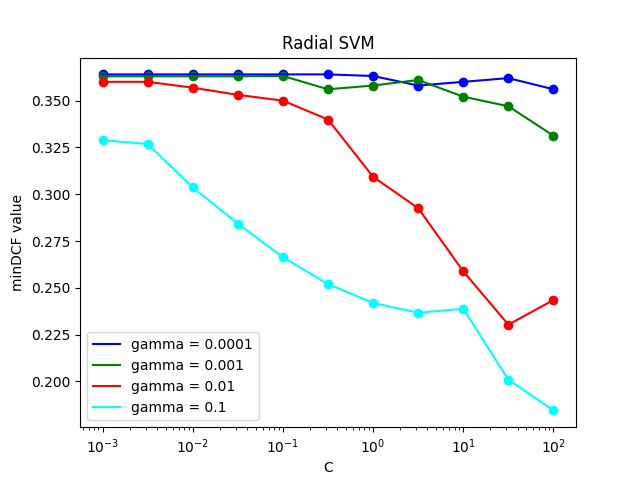
\includegraphics[width=\linewidth]{Lab/09. Lab 09/Images/07. Radial - minDCF}
        \label{fig:RadialminDCF}
    \end{subfigure}
    \begin{subfigure}[b]{0.40\linewidth}
        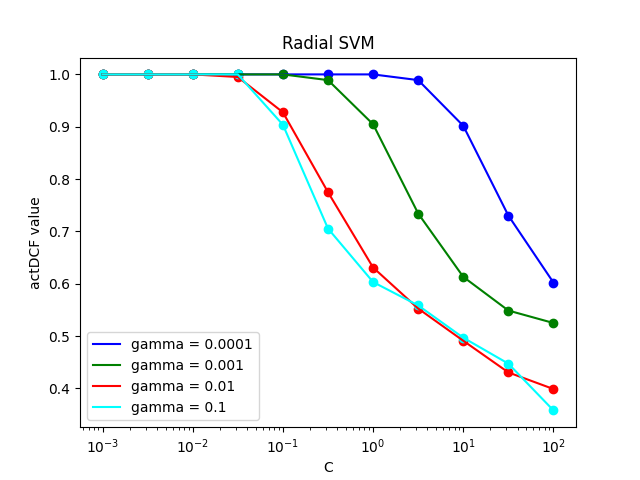
\includegraphics[width=\linewidth]{Lab/09. Lab 09/Images/08. Radial - actDCF}
        \label{fig:RadialactDCF}
    \end{subfigure}
    \caption{Shows minDCF and actDCF with polynomial kernel}
    \label{fig:RadialSVM}
\end{figure}

Now that this consideration has been made, we can specifically represent the values of minDCF and actDCF for values of \(\gamma=0.1\).
We can observe this result in \autoref{fig:RadialBestactDCF} and \autoref{tab:SVMRadialBest}.

\begin{figure}[h!]
    \centering
    \begin{subfigure}[b]{0.30\linewidth}
        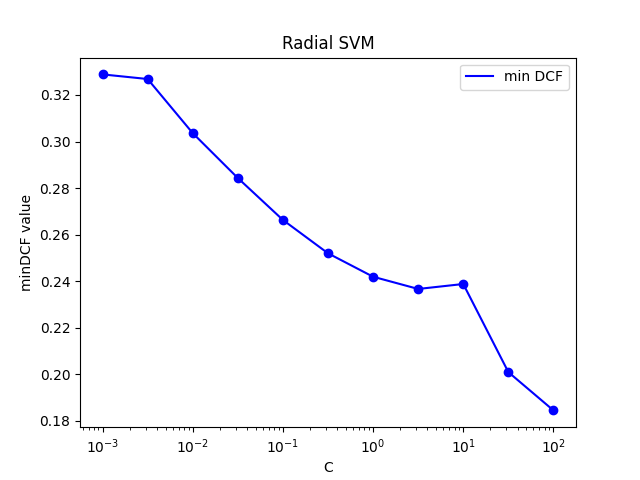
\includegraphics[width=\linewidth]{Lab/09. Lab 09/Images/09. Radial Best - minDCF}
        \label{fig:RadialBestminDCF}
    \end{subfigure}
    \begin{subfigure}[b]{0.30\linewidth}
        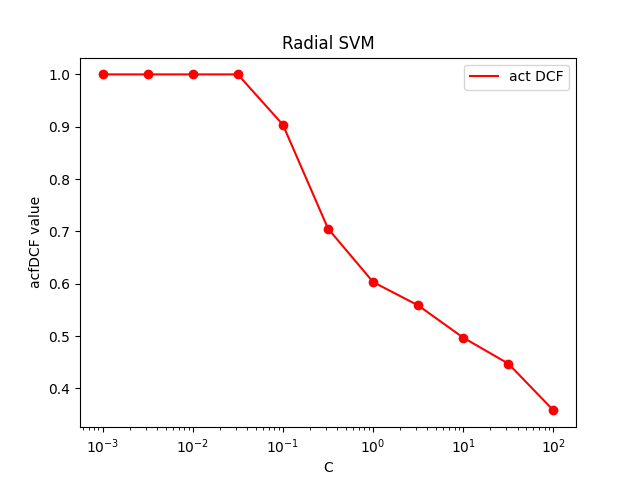
\includegraphics[width=\linewidth]{Lab/09. Lab 09/Images/10. Radial Best - actDCF}
        \label{fig:RadialBestactDCF}
    \end{subfigure}
    \begin{subfigure}[b]{0.30\linewidth}
        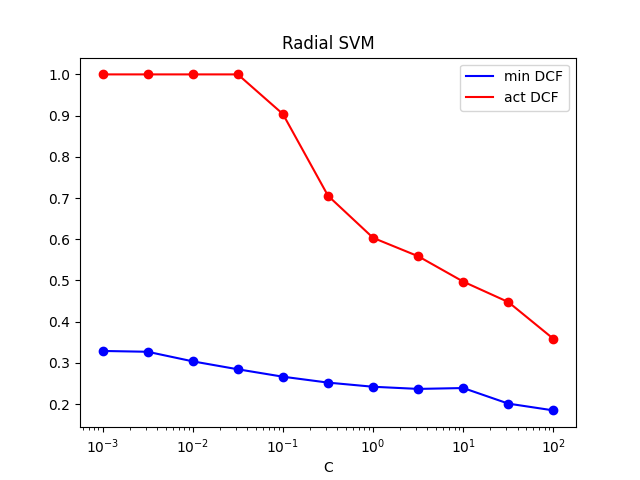
\includegraphics[width=\linewidth]{Lab/09. Lab 09/Images/11. Radial Best - min And actDCF}
        \label{fig:RadialBestminAndActDCF}
    \end{subfigure}
    \caption{Shows minDCF and actDCF with best RBF kernel}
    \label{fig:RadialBestSVM}
\end{figure}


\begin{table}[h!]
    \centering
    \begin{tabular}{>{\centering\arraybackslash}p{2.5cm} >{\centering\arraybackslash}p{2.5cm} >{\centering\arraybackslash}p{2.5cm}}
        \toprule
        \multicolumn{3}{c}{\textbf{Radial Kernel \(\xi = 1 \gamma = 0.1\)}} \\
        \midrule
        \texbf{C}   & \textbf{minDCF} & \textbf{actDCF} \\
        \midrule
        \(10^{-3}\) & 0.3288          & 1.0000          \\
        \(10^{-2}\) & 0.3036          & 1.0000          \\
        \(10^{-1}\) & 0.2663          & 0.9038          \\
        \(10^{0}\)  & 0.2419          & 0.6033          \\
        \(10^{1}\)  & 0.2388          & 0.4970          \\
        \midrule
        \multicolumn{3}{c}{\textbf{Best result}} \\
        \midrule
        \(10^{2}\)  & 0.1845          & 0.3581          \\
        \bottomrule
    \end{tabular}
    \captionsetup{justification=justified,singlelinecheck=false,format=hang}
    \caption{Show minDCF and actDCF for SVM with best RBF kernel}
    \label{tab:SVMRadialBest}
\end{table}

\bigskip
\textbf{Summarize}\par
Looking at the outcomes, one can see:
\begin{itemize}
    \item when parameter C increases, the outcomes become better and also better calibrated because the difference between minDCF and actDCF decreases.
    \item we can see that outcomes improve when switching from a linear to a polynomial kernel, which confirms what we have identified with QLR,
    namely modelling quadratic relationships between features to improve outcomes.
    \item the case with RBF kernels also confirms that more benefits can be gained from non-linear mapping
    \item As already mentioned, cases with higher C values improve outcomes and are better calibrated than cases with lower C values.
    But in general, a calibration operation could improve classification even for high C values.
\end{itemize}

